\chapter{Architecture}

\begin{figure}[h!]
\centering
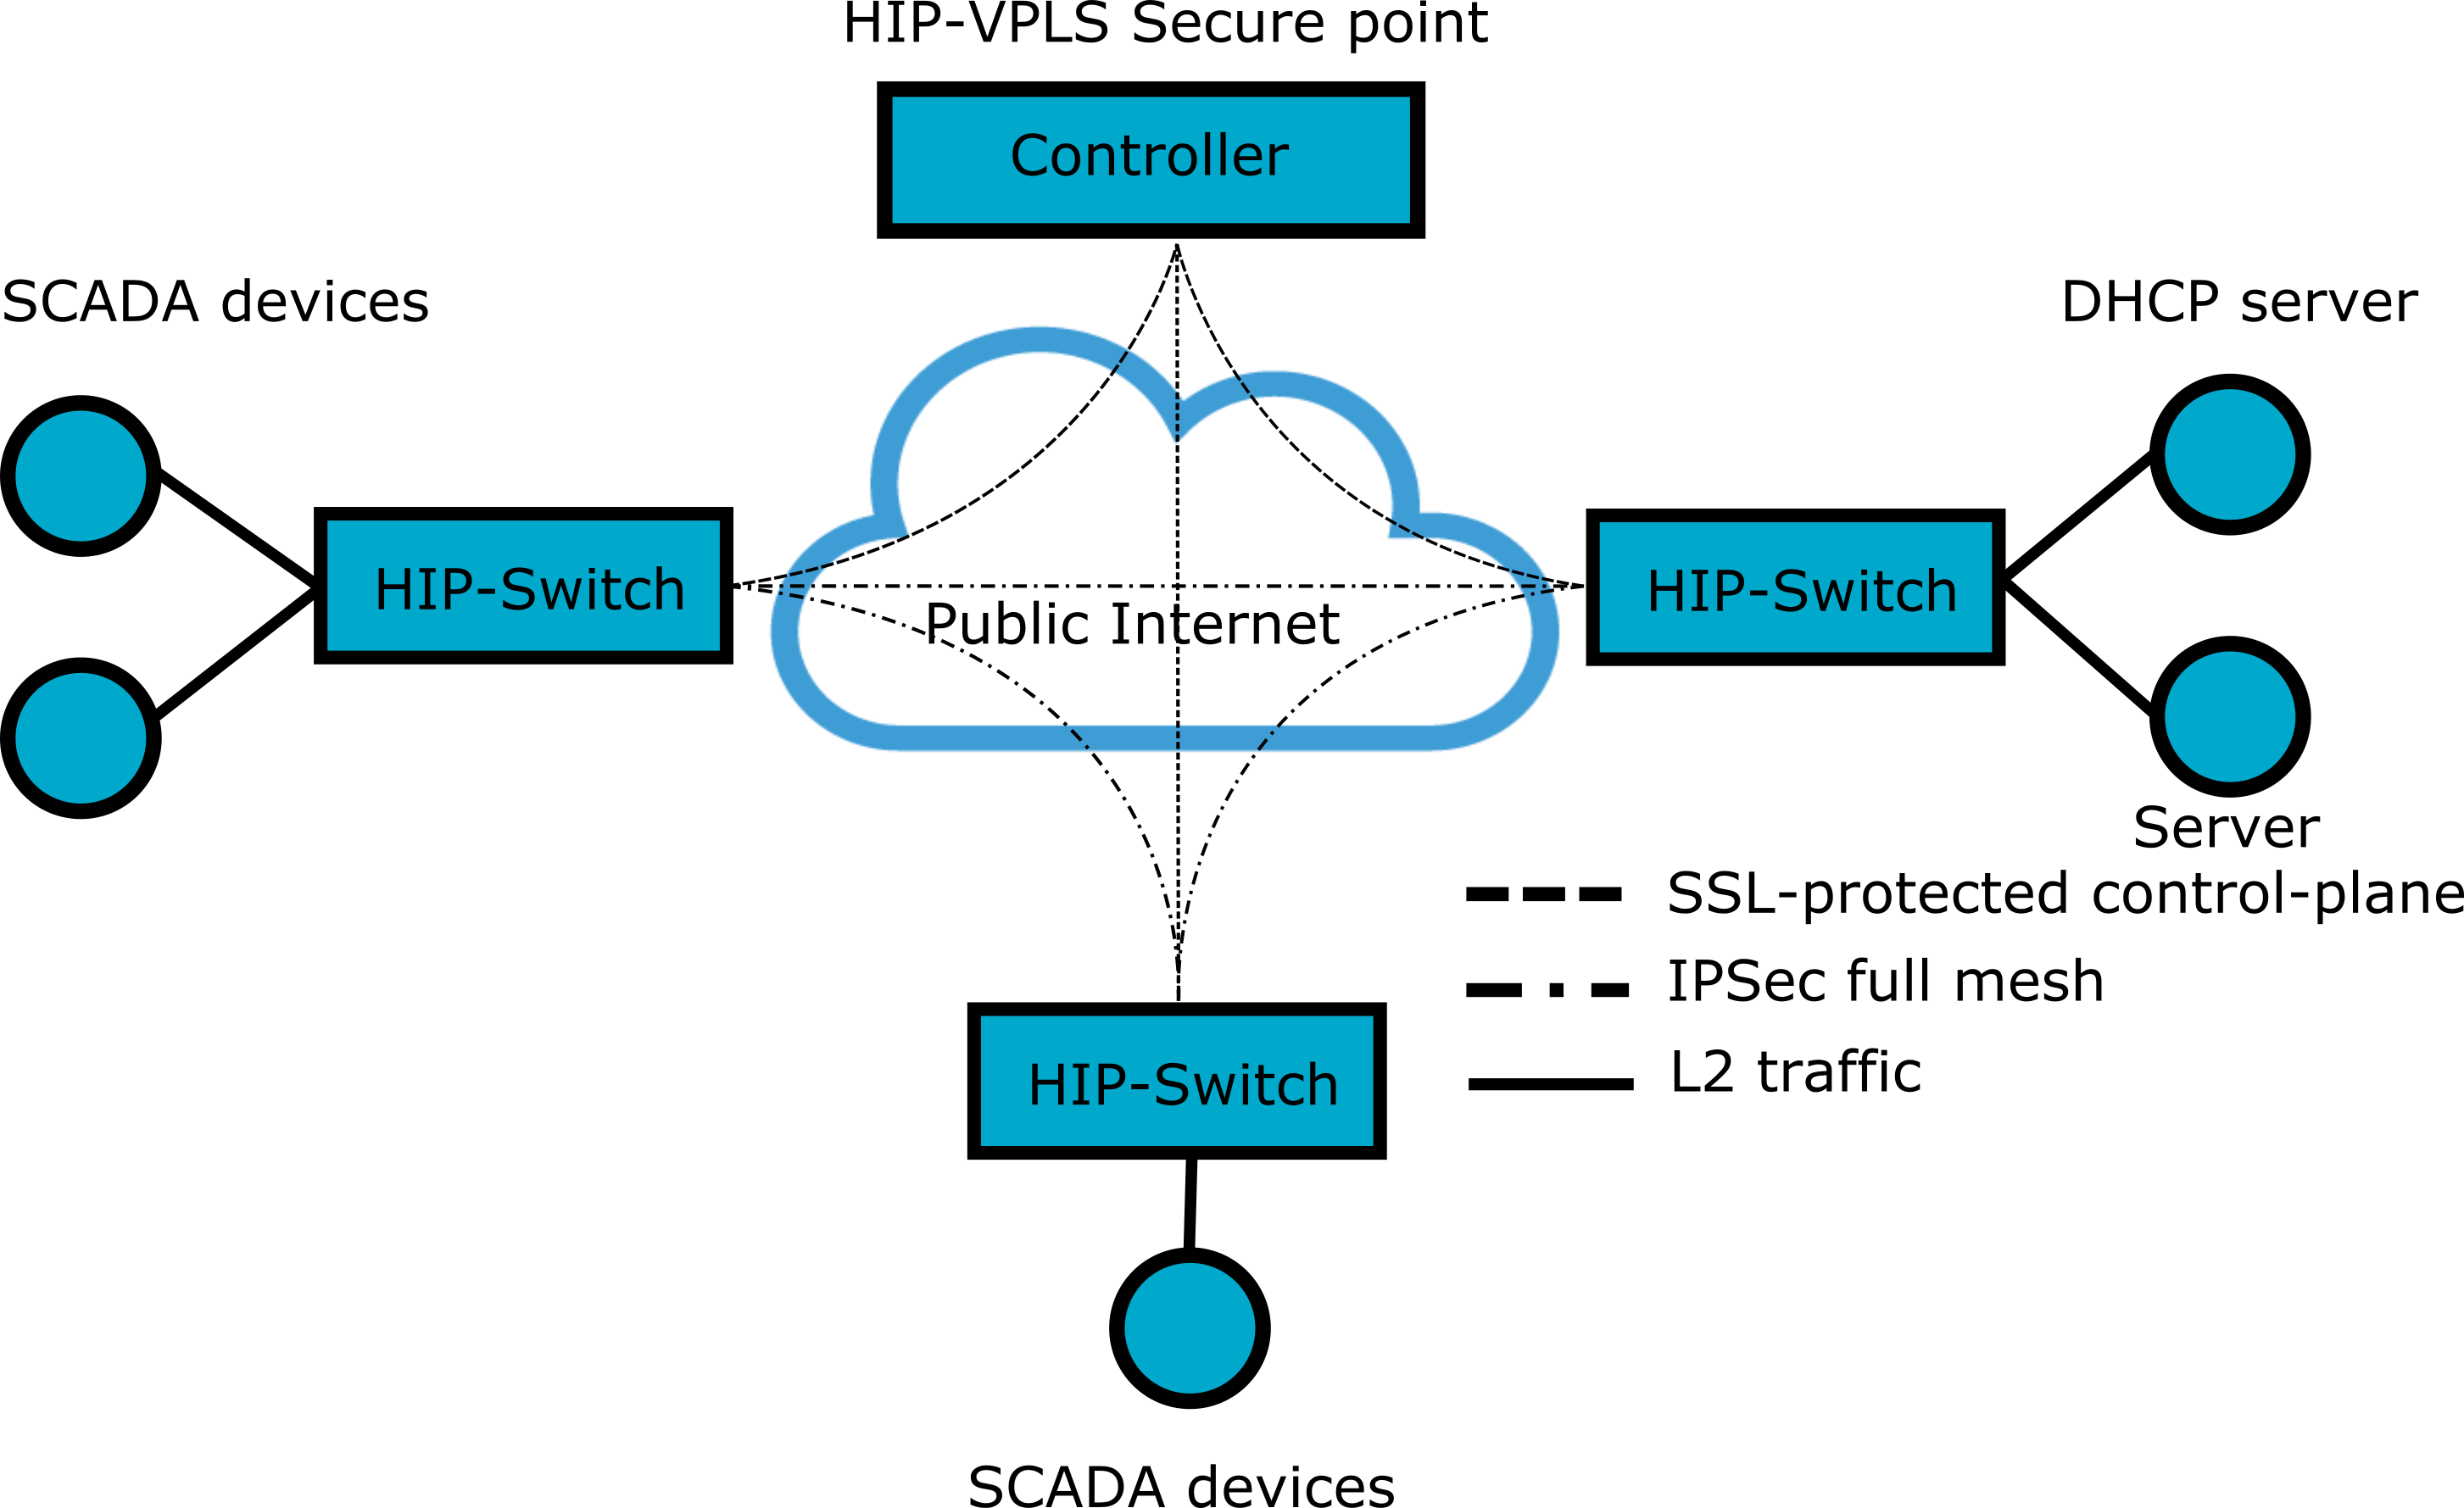
\includegraphics[width=0.9\textwidth]{graphics/arch.png}
\caption{System architecture}
\label{fig:architecture}
\end{figure}       


\begin{figure}[h!]
\centering
\includegraphics[width=0.9\textwidth]{graphics/testbed.png}
\caption{Testbed setup}
\label{fig:testbed}
\end{figure}       
    
\chapter{Proof-of-a-concept implementation}
In this chapter, we are going to discuss the proof of a concept
implementation of the HIP-VPLS (both HIP-switches and controller). 
In our work we have used the Python language as it offers simplicity
at the cost of extra CPU cycles to do the job.

\section{Accelerating AES with the hardware}

\section{Controller}
\subsection{HIP-switch registration}
\subsection{HIP-switch configuration}
\subsection{HIP-switch MAC Access Control List}
\subsection{HIP-switch traffic shaping}
Although we did not implement this feature in HIP-switches and HIP 
controller, we believe that it is still valuable for the future research.
For example, different hosts can be served differently (have more bandwidth)
than some other hosts by using traffic shaping. For example, if some hosts in HIP-VPLS 
network send delay sensitive traffic, for example, curtain rules can be configured 
on HIP controller to give needed advantage over other hosts in the network. We leave 
this for the future discussions and work.

\chapter{Performance evaluation}
Although our goal was not to build production grade solution
here we are still would like to discuss the performance 
(such as throughput) of our solution for two different settings:
(i) without optimizations (such as hardware AES acceleration) and 
without code improvements; and (ii) with the improvements. As the 
metric we are going to use user obtained throughput with iPerf tool. 

\begin{figure}[h!]
\centering
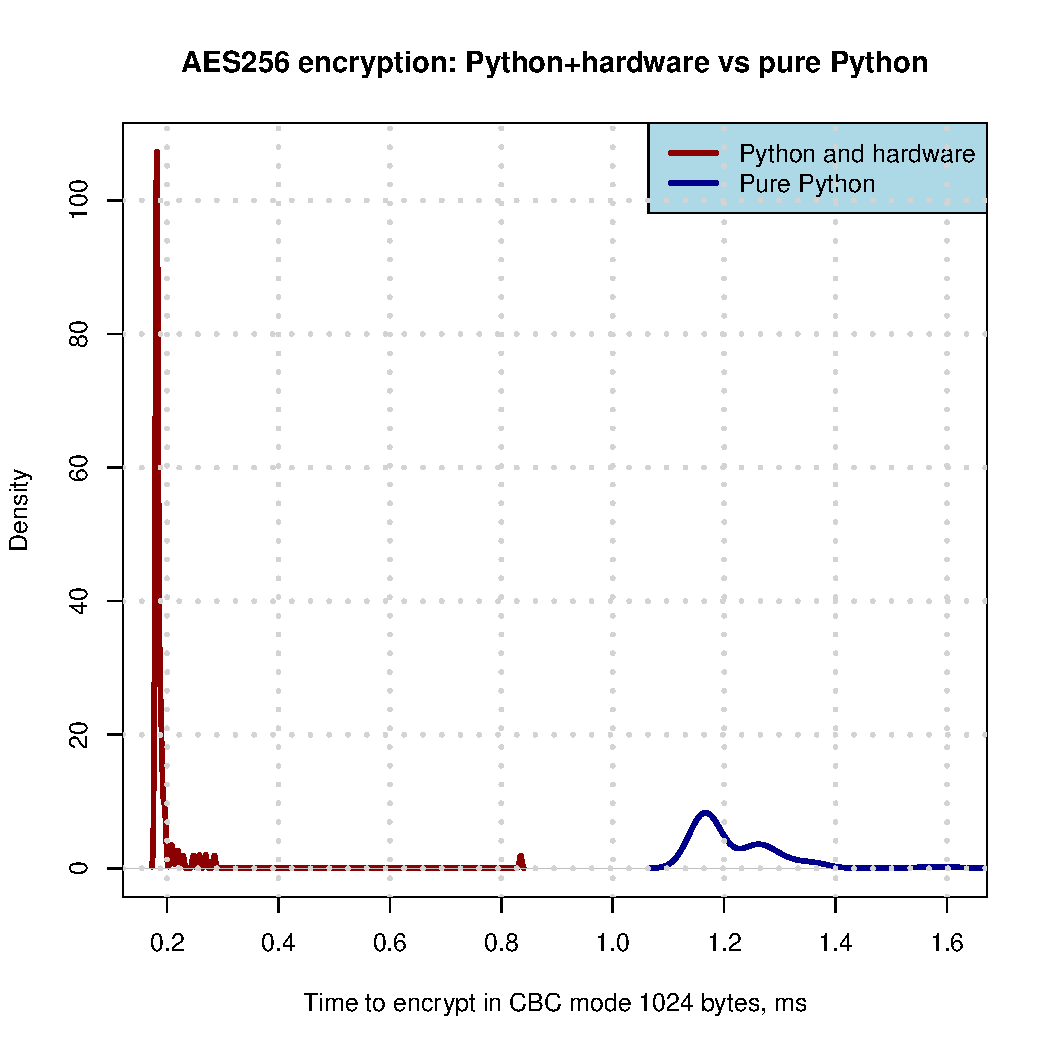
\includegraphics[width=0.9\textwidth]{graphics/AES.pdf}
\caption{AES encrption perfromance}
\label{fig:testbed}
\end{figure}
